\chapter{プロダクト}

\section{アプリケーションのコンセプト}
BuLoは,バスに乗り遅れたくないがバスを効率的に使いたいひとのためのバスロケーションアプリである.
従来のバスロケーションアプリやGoogle Mapsなどの地図アプリとは異なり,バスの位置や遅延情報をリアルタイムにわかりやすく把握することができる.
また,本サービスは``ひとめぼれ''するバスロケーションアプリをめざしている.我々は``ひとめぼれ''を以下の2つと考える.
まず1つ目にアプリのデザインに対する``ひとめぼれ''である.これは本サービスを使うきっかけとなるものである.
2つ目にアプリ全体を通しての体験への``ひとめぼれ''である.これは本サービスを使い続けるきっかけになると考える.
\bunseki{下村蒔里萌}

\section{機能}
\subsection{住所を登録}
本サービスは自宅と職場の住所を登録する機能を搭載している.
対象ユーザは通勤・通学にバスを利用する人であり,使用するルートは変わらないことが予測できるため,最初に住所を登録をすることで2回目以降は再度住所の検索をする手間を省いている.
図\ref{fig:feature_register}の左から3枚目の画面では,現在地の住所をサジェストしている.
住所の入力では,キーワードに対しての予測をサジェストしている.
\begin{figure}[H]
    \centering
    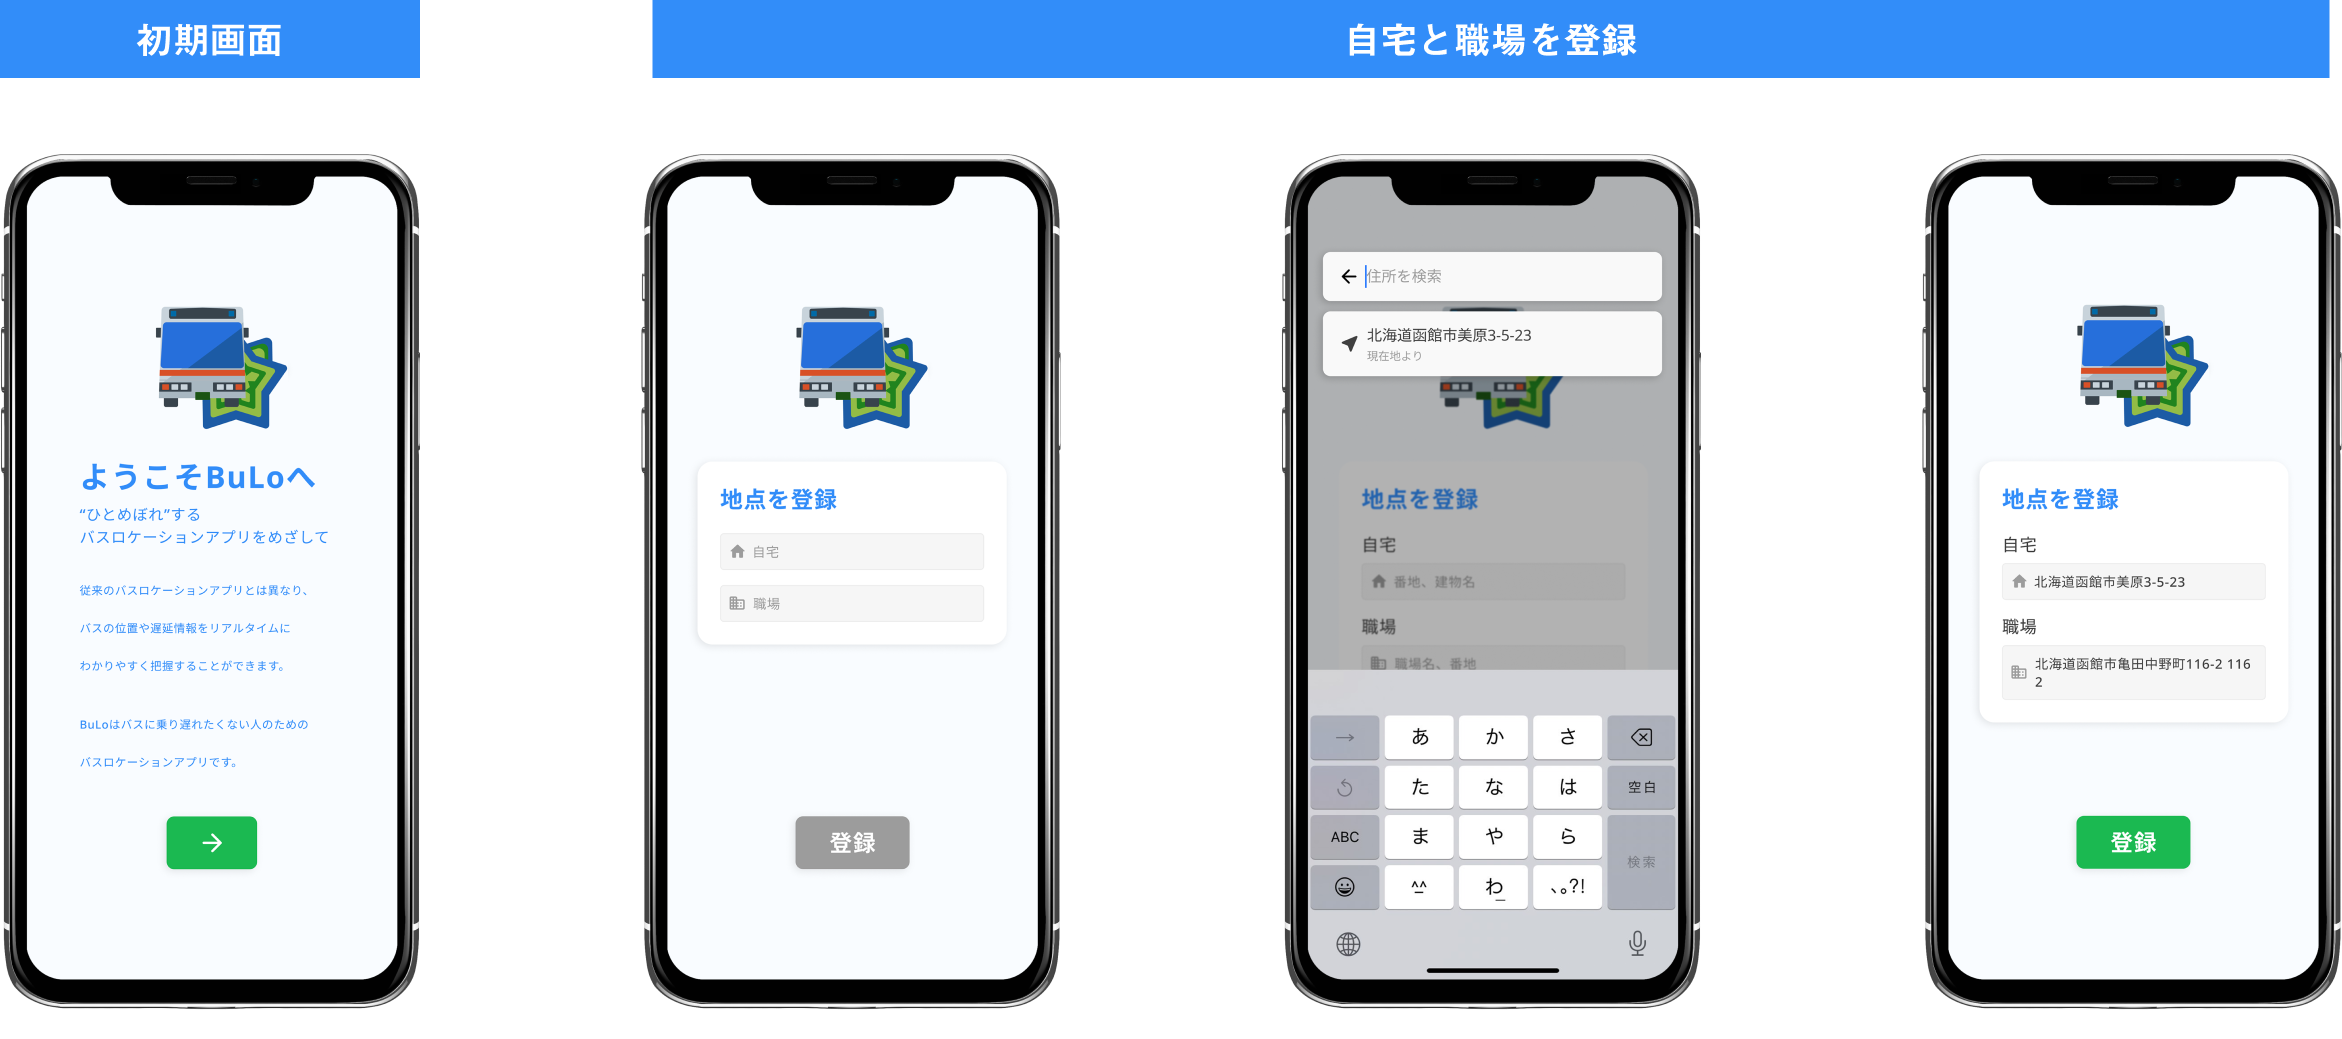
\includegraphics[width=14cm]{images/feature_register.png}
    \caption{住所を登録}
    \label{fig:feature_register}
\end{figure}
\subsection{Time-Distance ListとRoute View}
ユーザが住所を登録したあと,ユーザがアプリを開いた際は図\ref{fig:feature_td}の画面を表示する.
図\ref{fig:feature_td}の左側の画面は,後述するTime-Distance Viewの一覧である.
一覧は,バスがユーザの乗車するバス停に到着する順に表示される.
図\ref{fig:feature_td}の右側の画面は,各Time-Distance Viewをタップした際に表示されるRoute Viewである.
ここではタップしたTime-Distance Viewと,ユーザとそのバスの現在地がマップ上に表示される.
\begin{figure}[H]
    \centering
    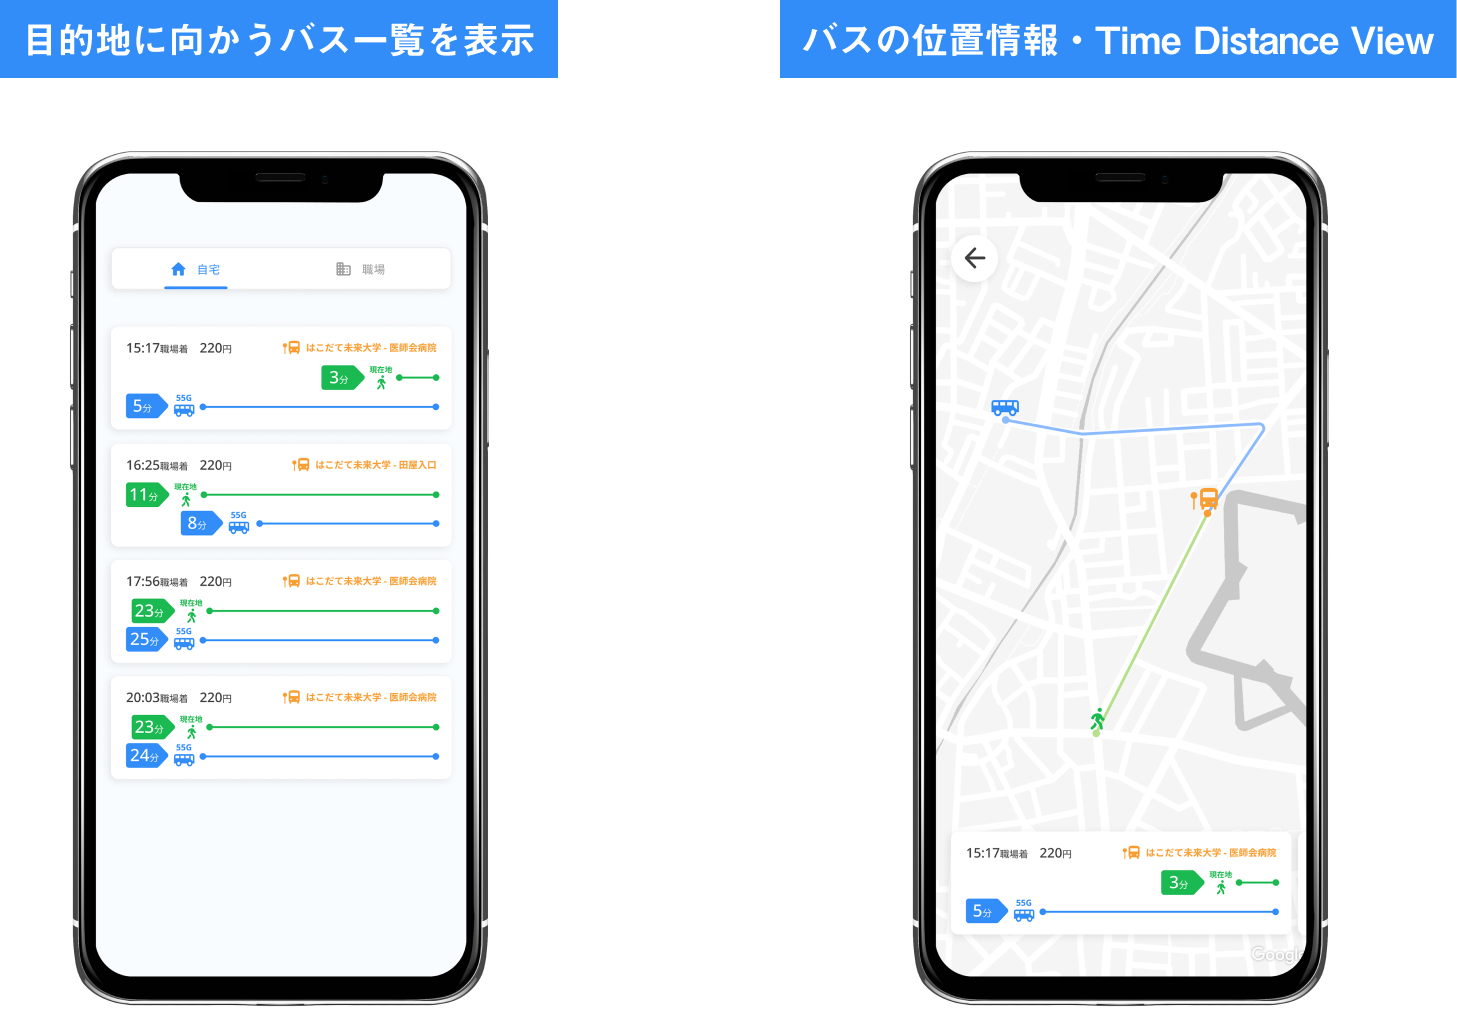
\includegraphics[width=14cm]{images/feature_td.png}
    \caption{Time-Distance ViewとRoute View}
    \label{fig:feature_td}
\end{figure}
\subsection{Time-Distance Viewの詳細}
Time-Distance Viewとは,ユーザの現在地・バスの現在地・バス停の3点を時間的グラフに表したものである.
これにより,ユーザは「バスに間に合うかどうか」,「バス停でどのくらい待つか」がひとめでわかる.
実装方法は図\ref{fig:feature_timedistanceview}に示す.
また,図\ref{fig:feature_timedistanceview}では以下の状況を考えている.
\begin{quote}
    \begin{itemize}
        \item ユーザの目的地は自宅(田家入口の近く)
        \item 現在地からの最寄りのバス停ははこだて未来大学駅
        \item ユーザが乗るバスは55G
        \item ユーザが自宅に行くまでにかかる料金は220円
        \item バスは5分後にはこだて未来大学駅に到着する
        \item 現在地からはこだて未来大学駅まで徒歩で3分かかる
        \item 自宅には16:25に到着する
    \end{itemize}
\end{quote}
\begin{figure}[H]
    \centering
    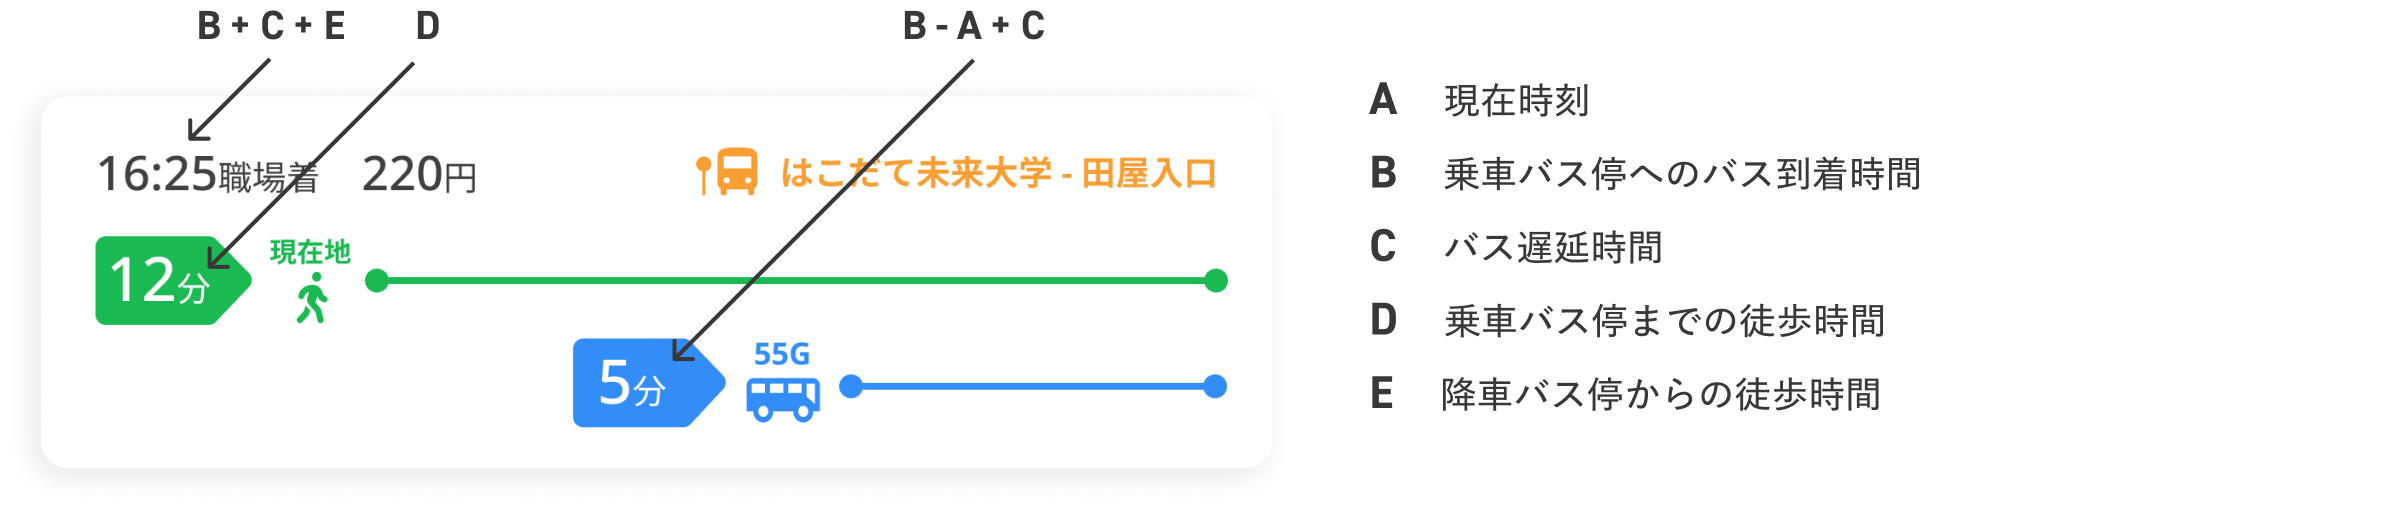
\includegraphics[width=14cm]{images/feature_timedistanceview.png}
    \caption{Time-Distance View}
    \label{fig:feature_timedistanceview}
\end{figure}
図\ref{fig:feature_timedistanceview2}では,想定されるTime-Distance Viewの例を示している.
図\ref{fig:feature_timedistanceview2}の左から,「ユーザがバスに安心して乗れる状態」
「ユーザがバス停でかなり待つことが予想できるため,バス停以外の場所で時間をつぶすことができる」
「ユーザよりバスの方が先にバス停に到着するが,走ることでバスに乗ることができる」状態である.
\begin{figure}[H]
    \centering
    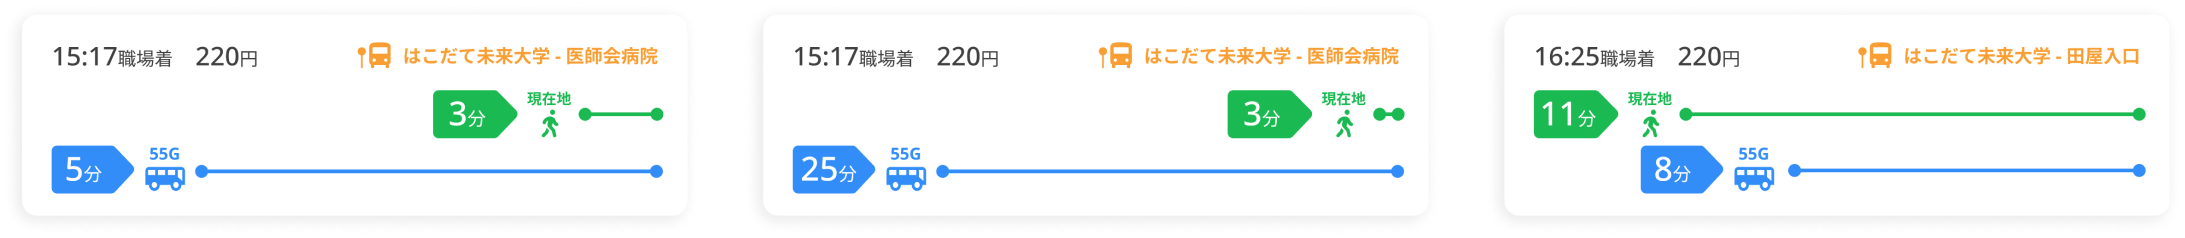
\includegraphics[width=14cm]{images/feature_timedistanceview2.png}
    \caption{Time-Distance Viewの例}
    \label{fig:feature_timedistanceview2}
\end{figure}
\bunseki{下村蒔里萌}

\section{デザインシステム}
本サービスでは,デザインシステムを導入している.
Colors,Typographies,Icons,Shapes and Othersの4つのカテゴリに分けて,デザインシステムを構築した.
\subsection{Colors}
本サービスのカラーパレットは図\ref{fig:feature_colors}のように設定した.
16進数のカラーコード(例: \#FF3B30)に具体的な値を与え使いやすくしたプリミティブトークン(例: red)と,
特定の用途別に定義したセマンティックトークン(例: alert)を定義している.
Figma上でのプロトタイプや実装では,セマンティックトークンを使用した.
\begin{figure}[H]
    \centering
    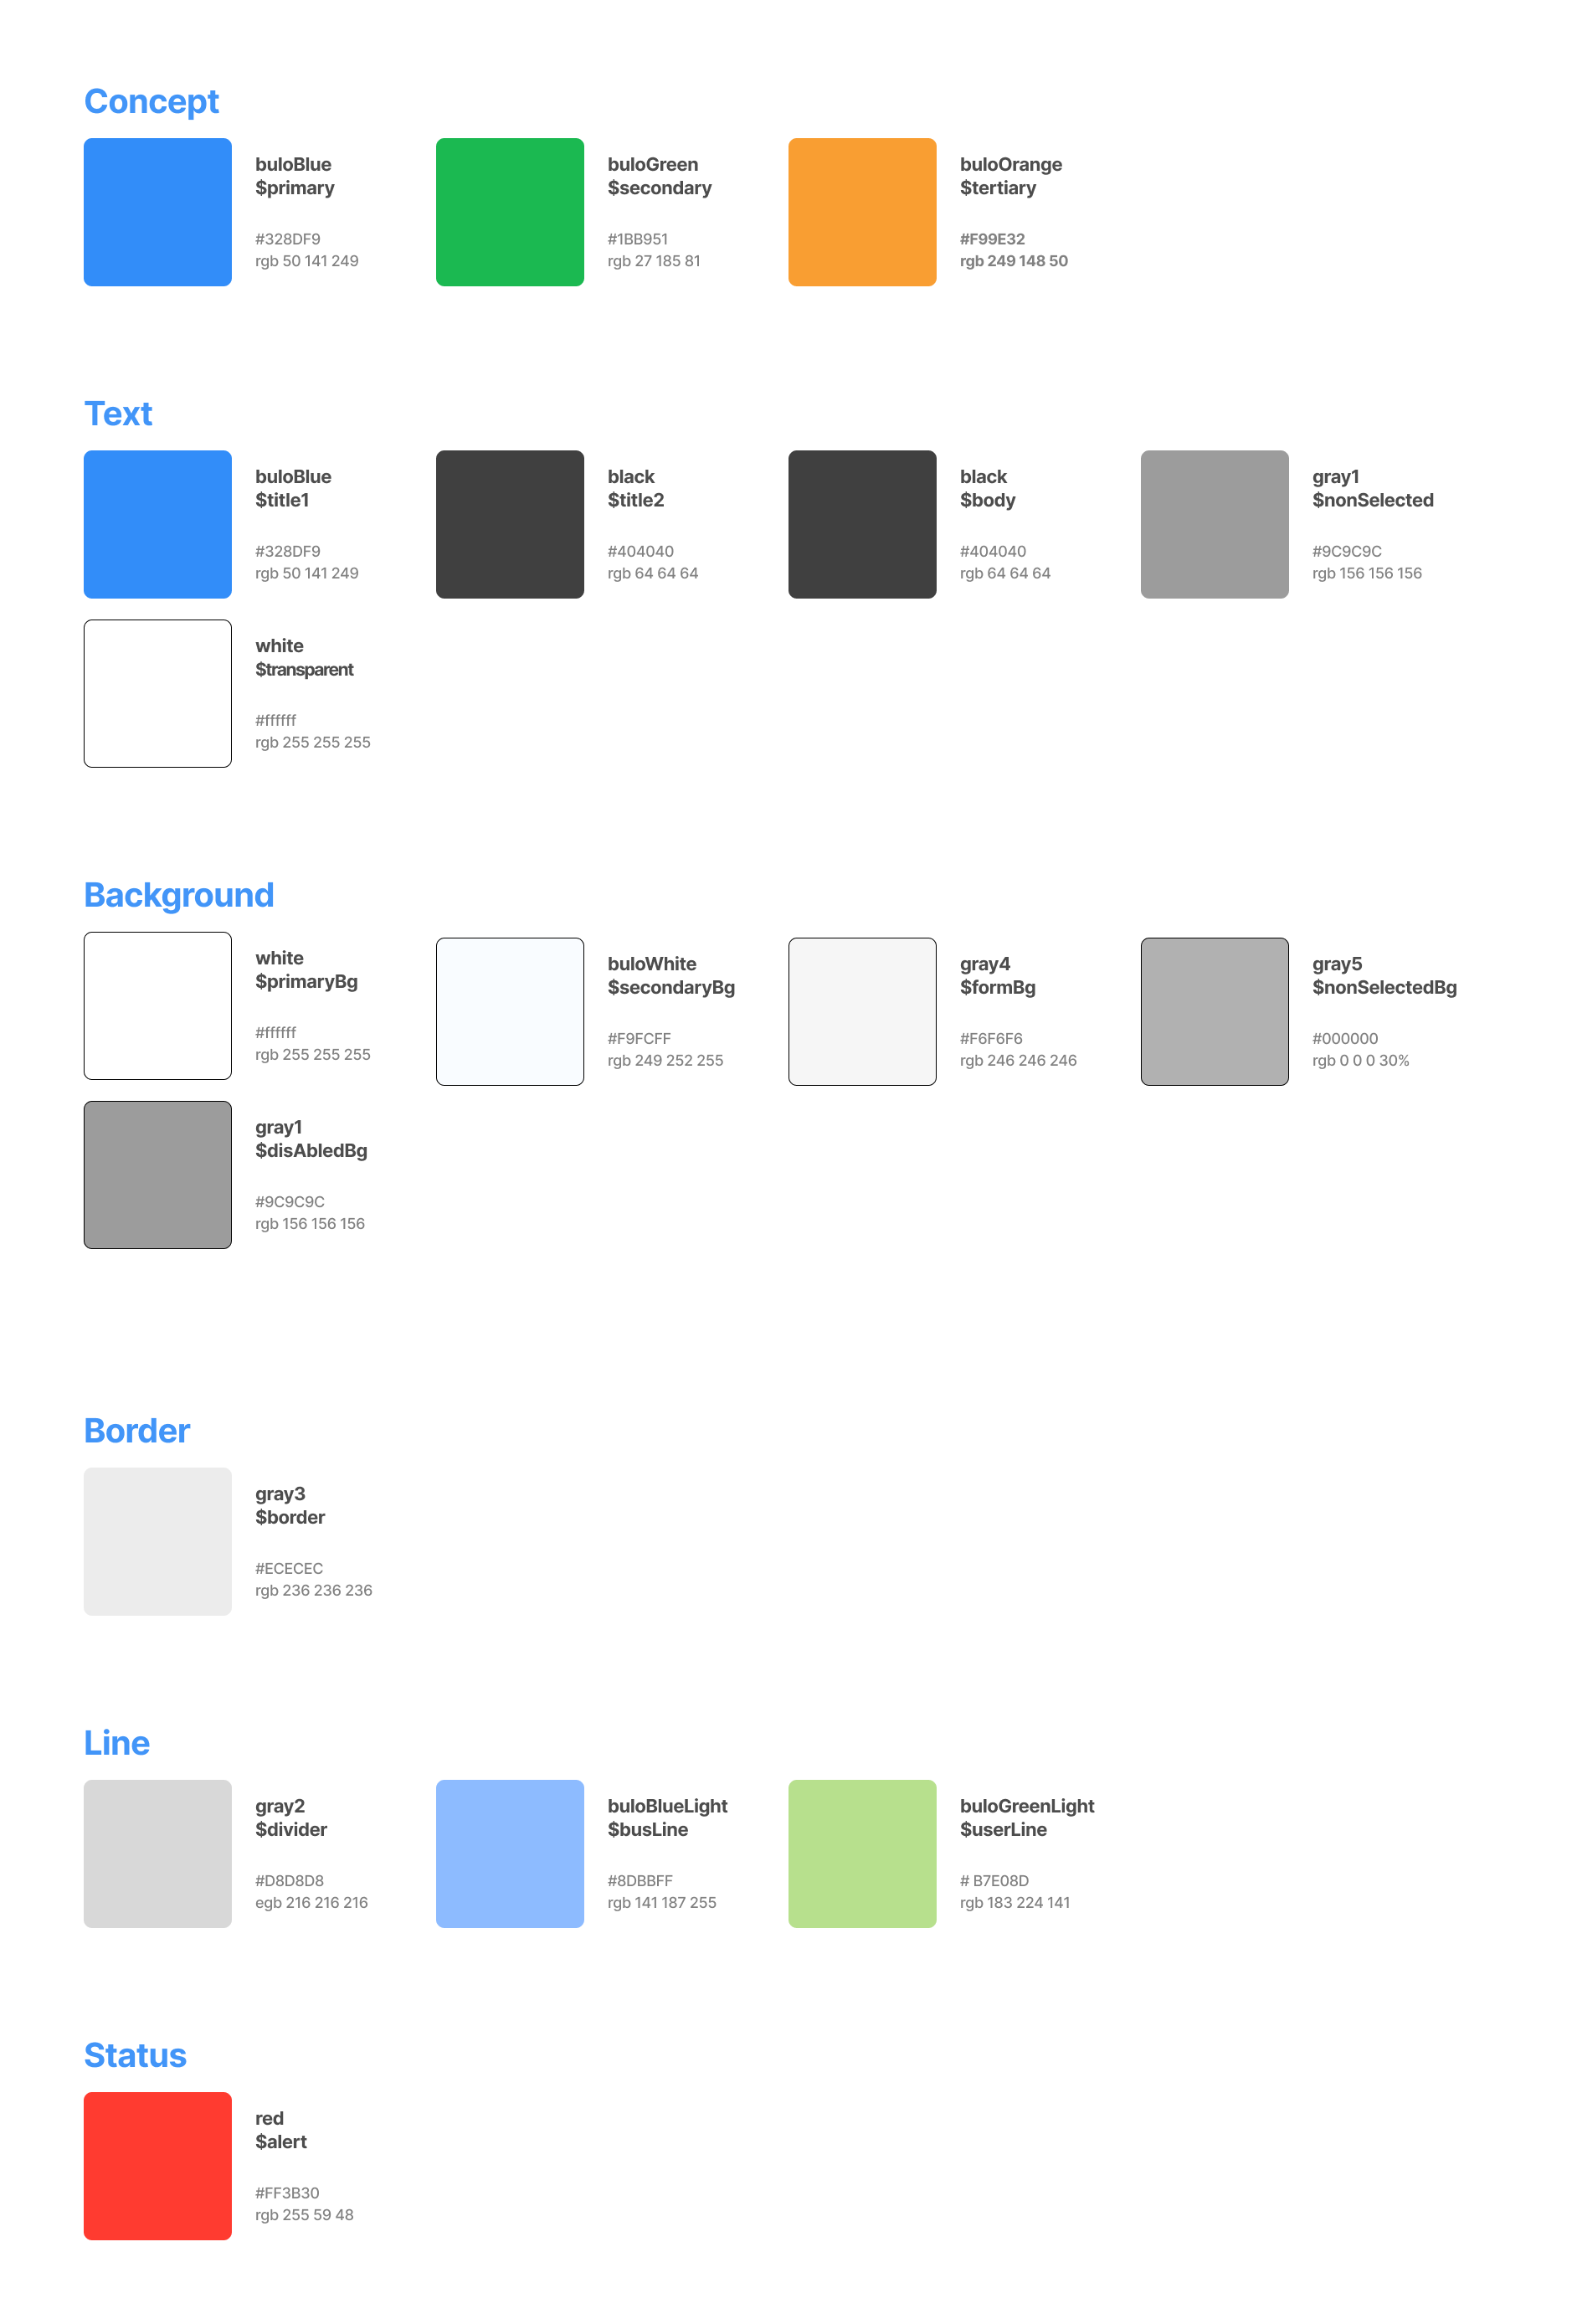
\includegraphics[width=12cm]{images/colors.png}
    \caption{デザインシステム Colors}
    \label{fig:feature_colors}
\end{figure}
\subsection{Typographies}
本サービスのフォントは図\ref{fig:typographies}のように設定した.
\begin{figure}[H]
    \centering
    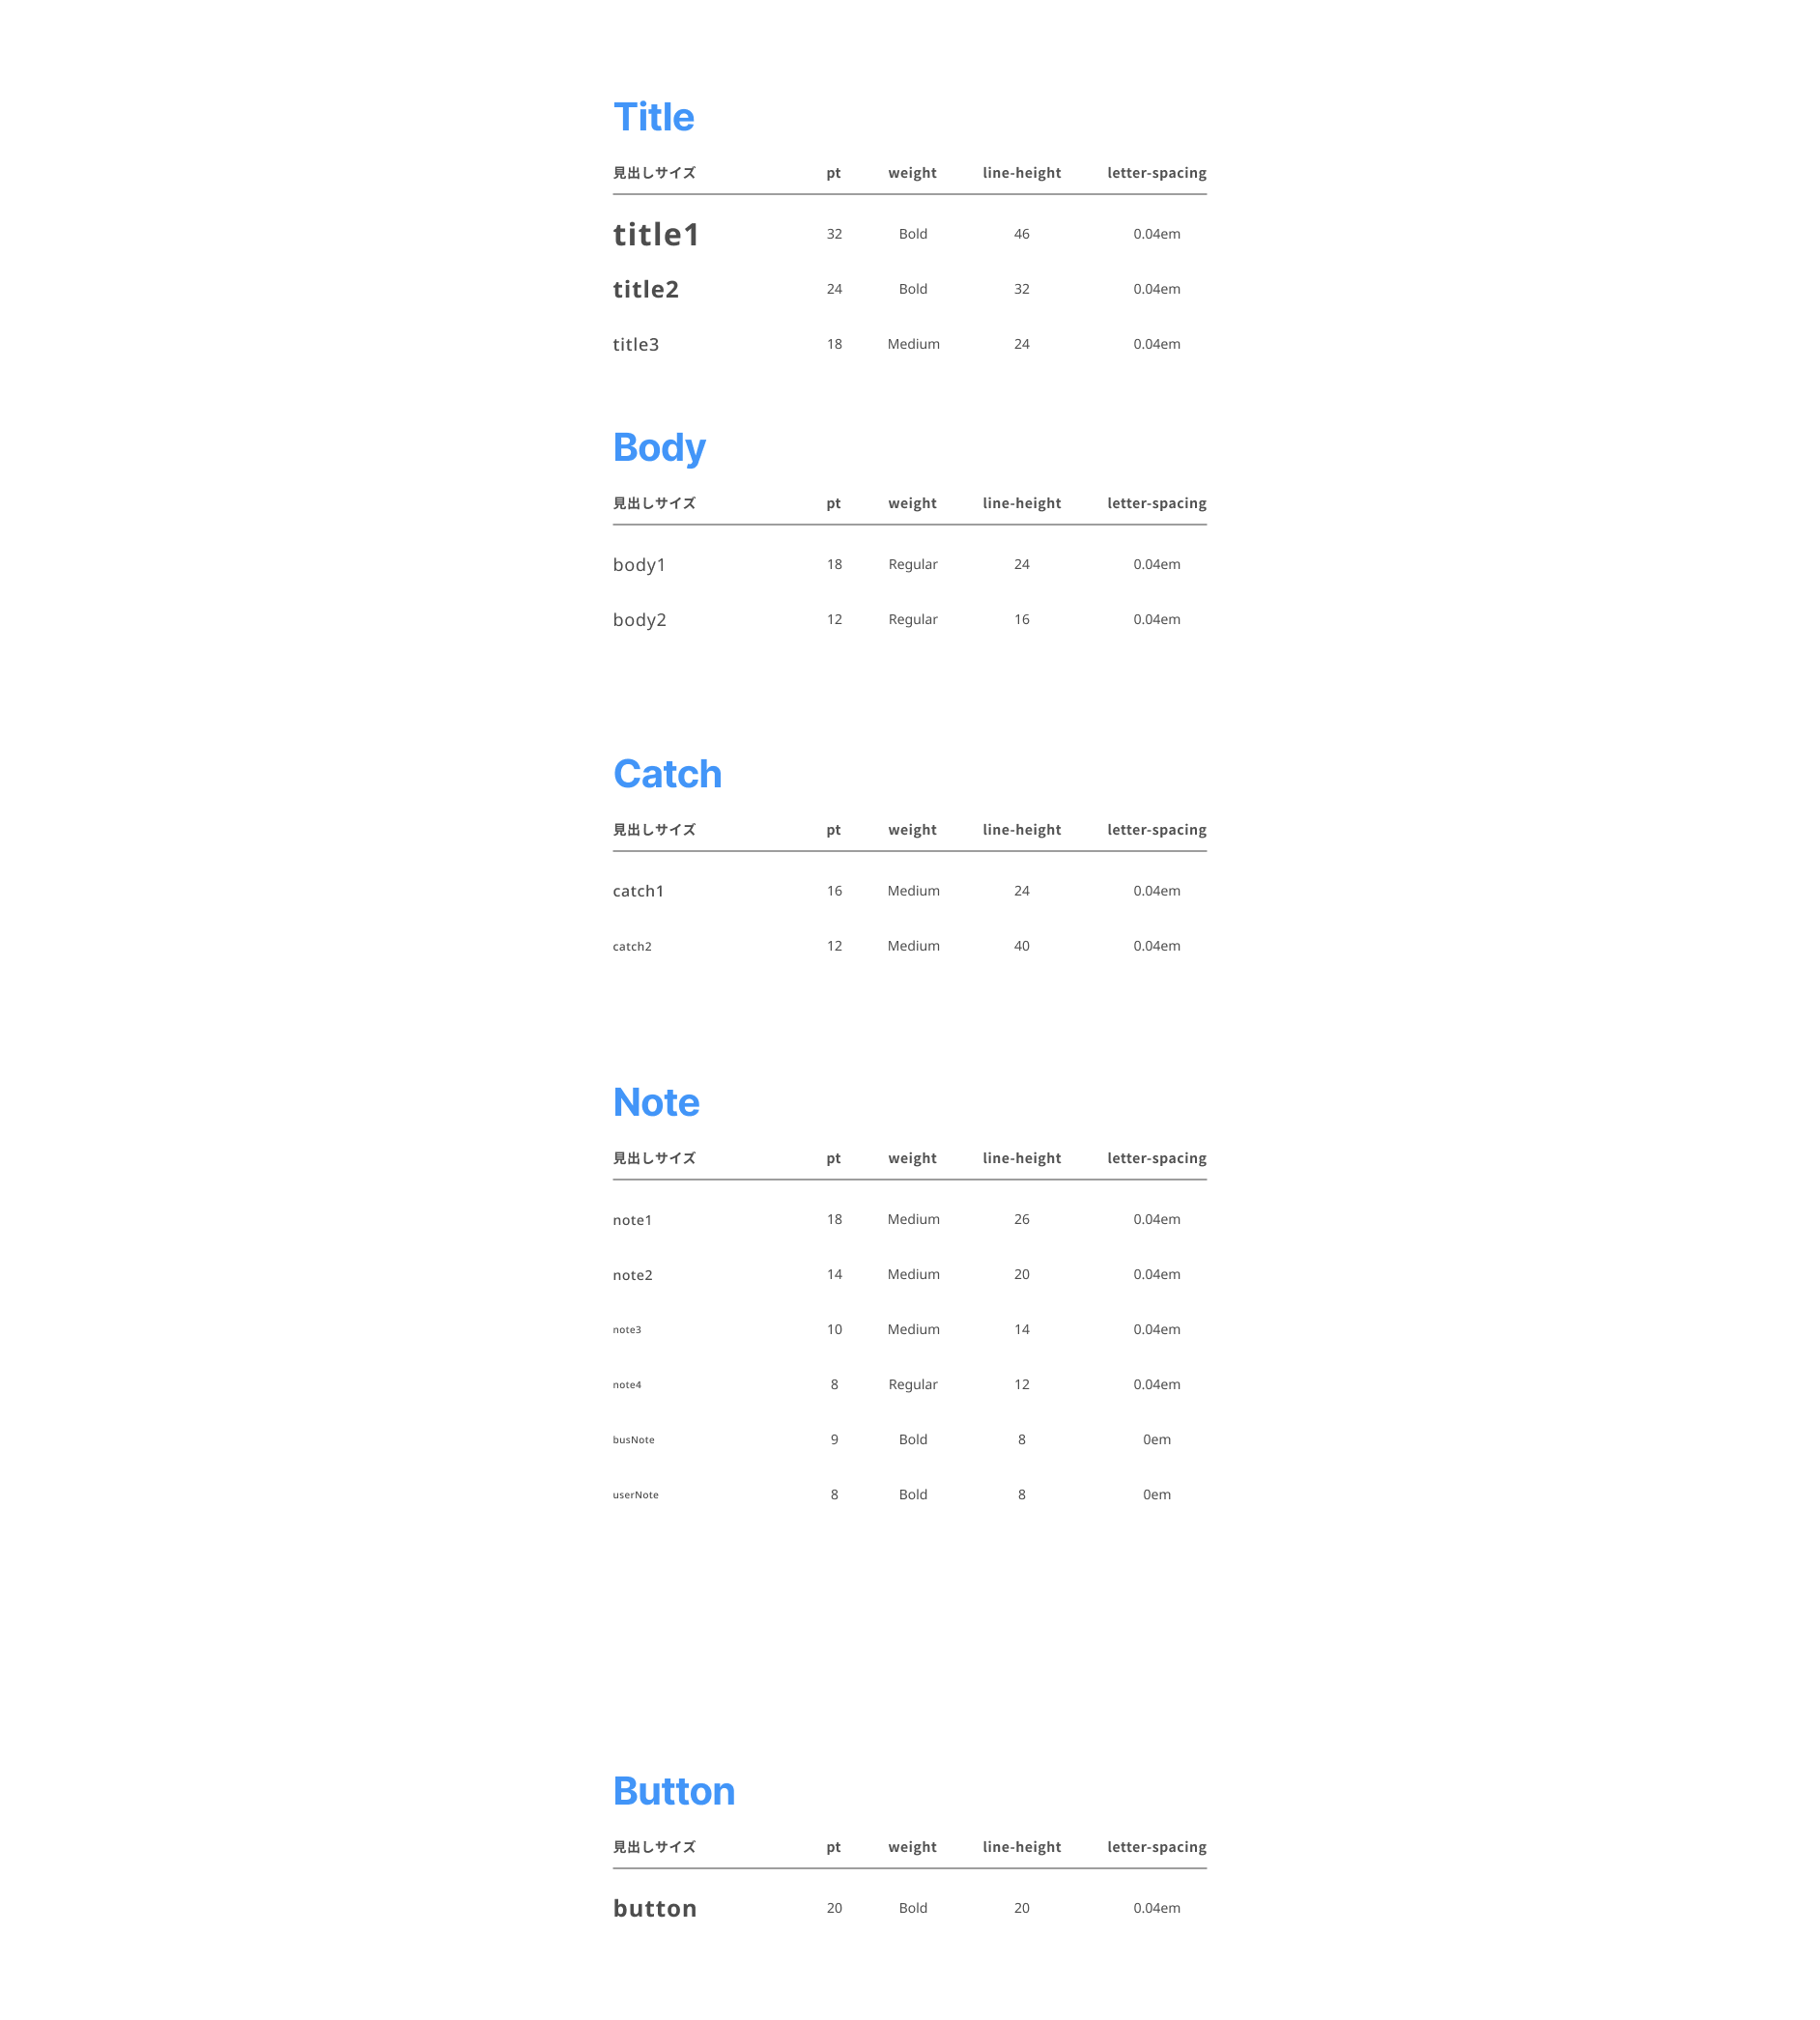
\includegraphics[width=7cm]{images/typographies.png}
    \caption{デザインシステム Typographies}
    \label{fig:typographies}
\end{figure}
\subsection{Icons}
    本サービスのアイコンは図\ref{fig:icons}のように設定した.
    主にMaterial Symbols and Icons\footnote{https://fonts.google.com/icons}を使用し,足りないものはPictogrammers\footnote{https://pictogrammers.com/}を使用した.
        \begin{figure}[H]
            \centering
            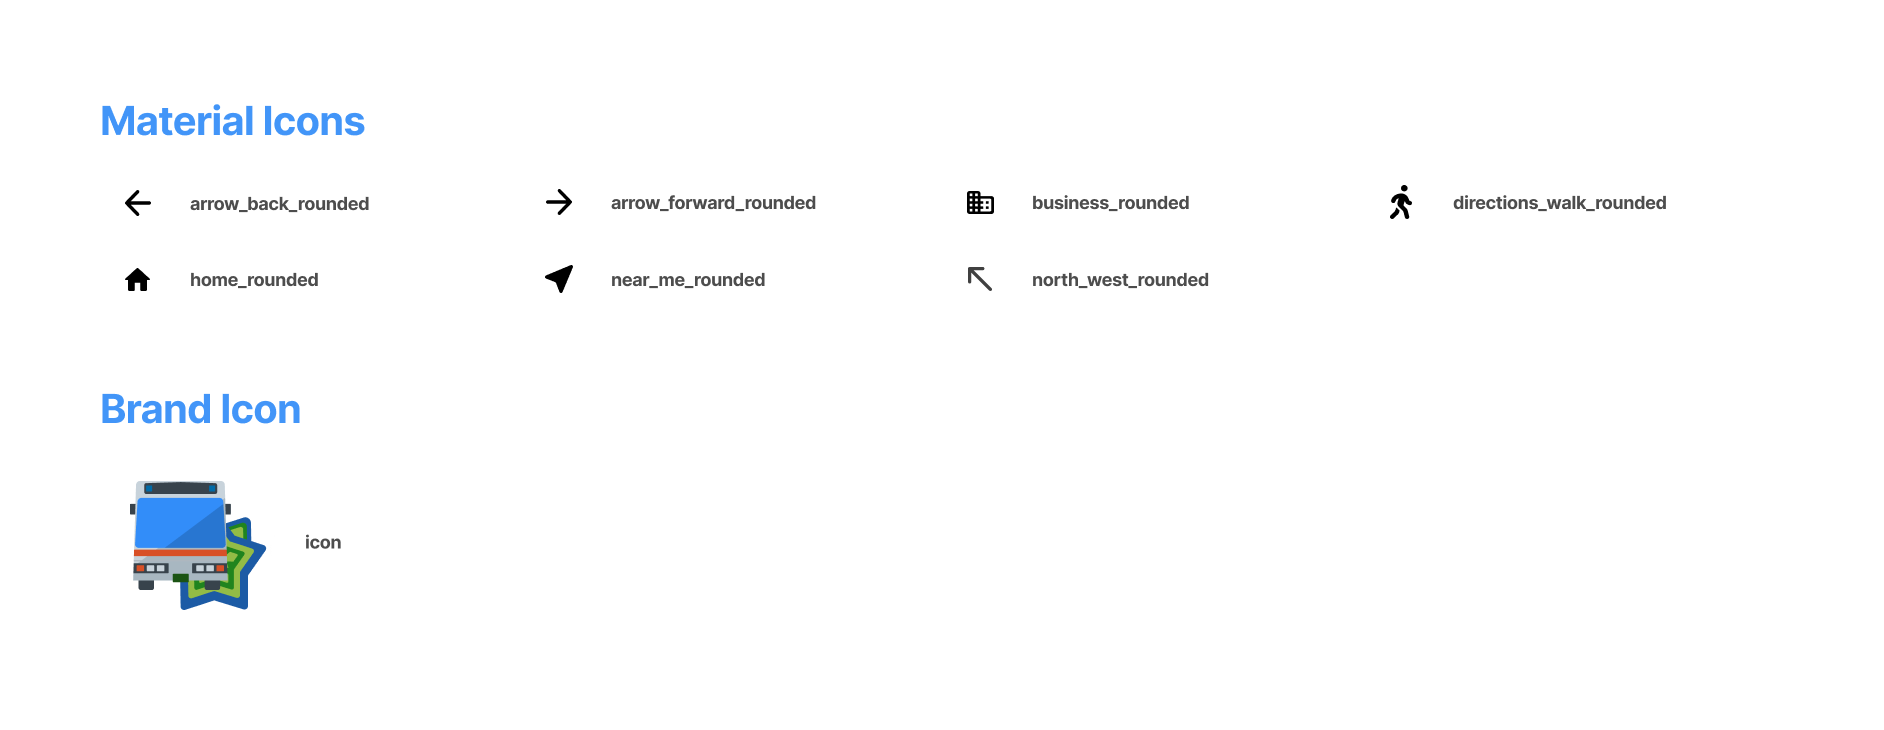
\includegraphics[width=14cm]{images/icons.png}
            \caption{デザインシステム Icons}
            \label{fig:icons}
        \end{figure}
\subsection{Shapes and Others}
    本サービスの形状とその他のデザインは図\ref{fig:shapes}のように設定した.
    ElevationやBlurは2つのレイヤー間のz軸上の深度を表す.
    インターフェイス上の最も上位の要素をより強調することで,アクションの重要度を伝える.
    Cornersは角丸を表し,4, 8, 16と3種類の数字を用意し,コンポーネントの短辺に合わせて角丸の数値を可変する.
    角丸を使用した図形の中に,角丸を使用した図形位がある場合は,
    外側の図形の角丸=内側の図形の角丸+内側の余白とする.
\begin{figure}[H]
    \centering
    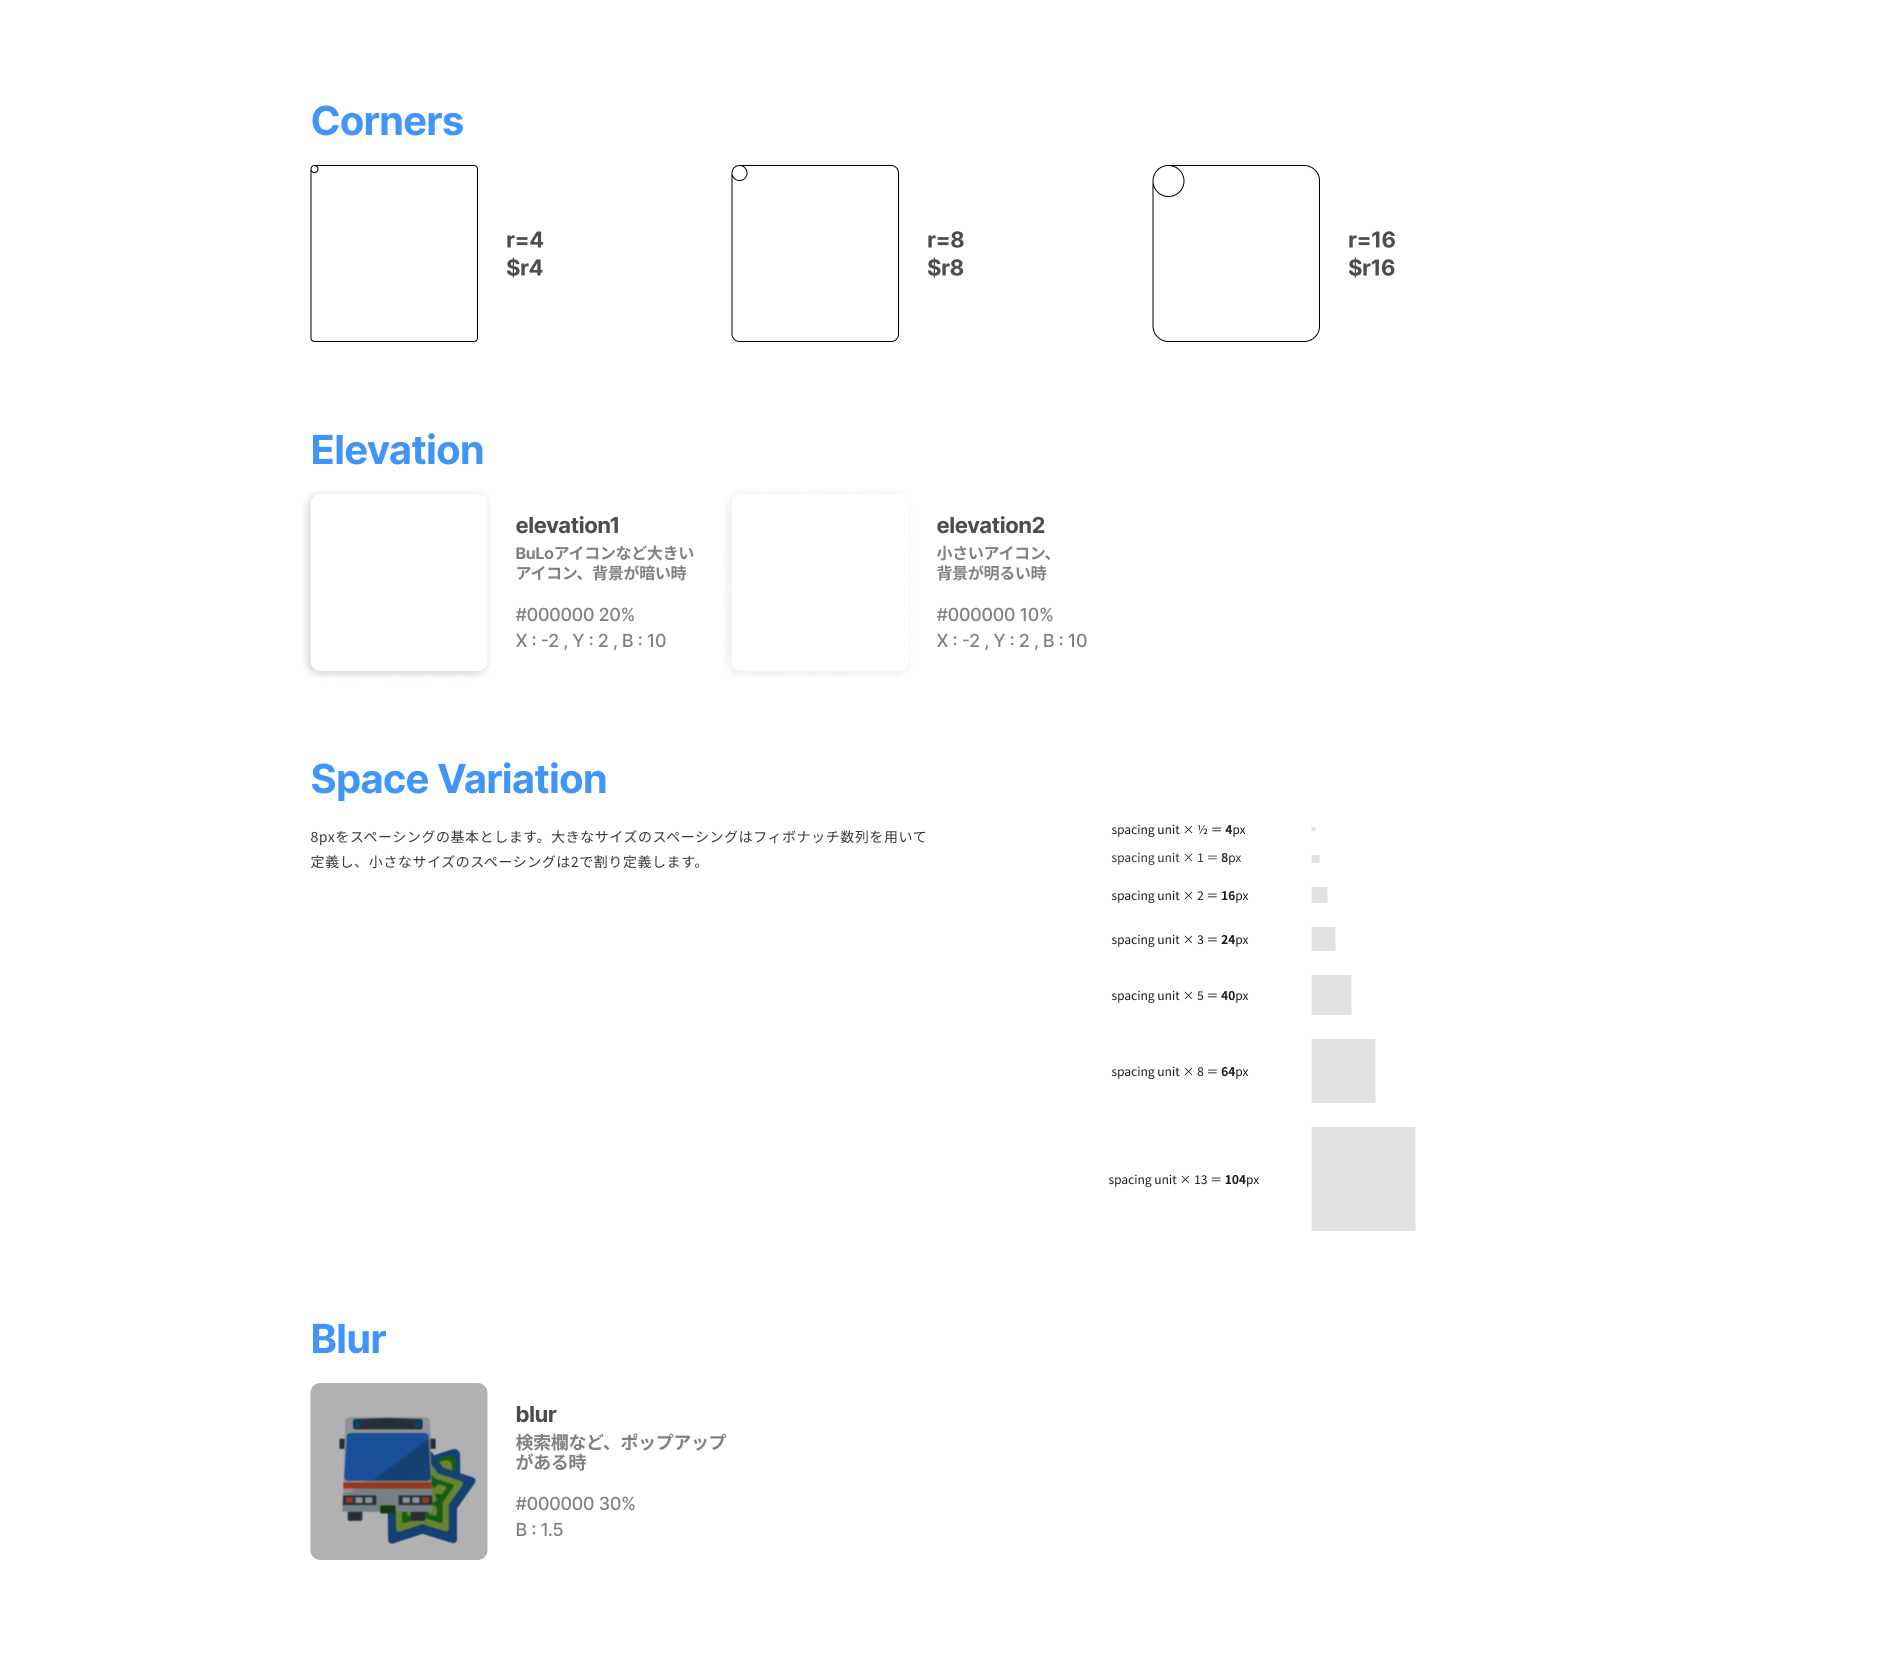
\includegraphics[width=14cm]{images/shapes.png}
    \caption{デザインシステム Shapes and Others}
    \label{fig:shapes}
\end{figure}
\bunseki{下村蒔里萌}

\section{システムの構成}
本サービスでは,マイクロサービスアーキテクチャを採用している.クライアントは,BFF (Backend for Frontend) を介して,バックエンドのマイクロサービスと通信する.
バックエンドのマイクロサービス間は,gRPCを用いて通信する.アーキテクチャ図を図\ref{fig:architecture}に示す.
\begin{figure}[H]
    \centering
    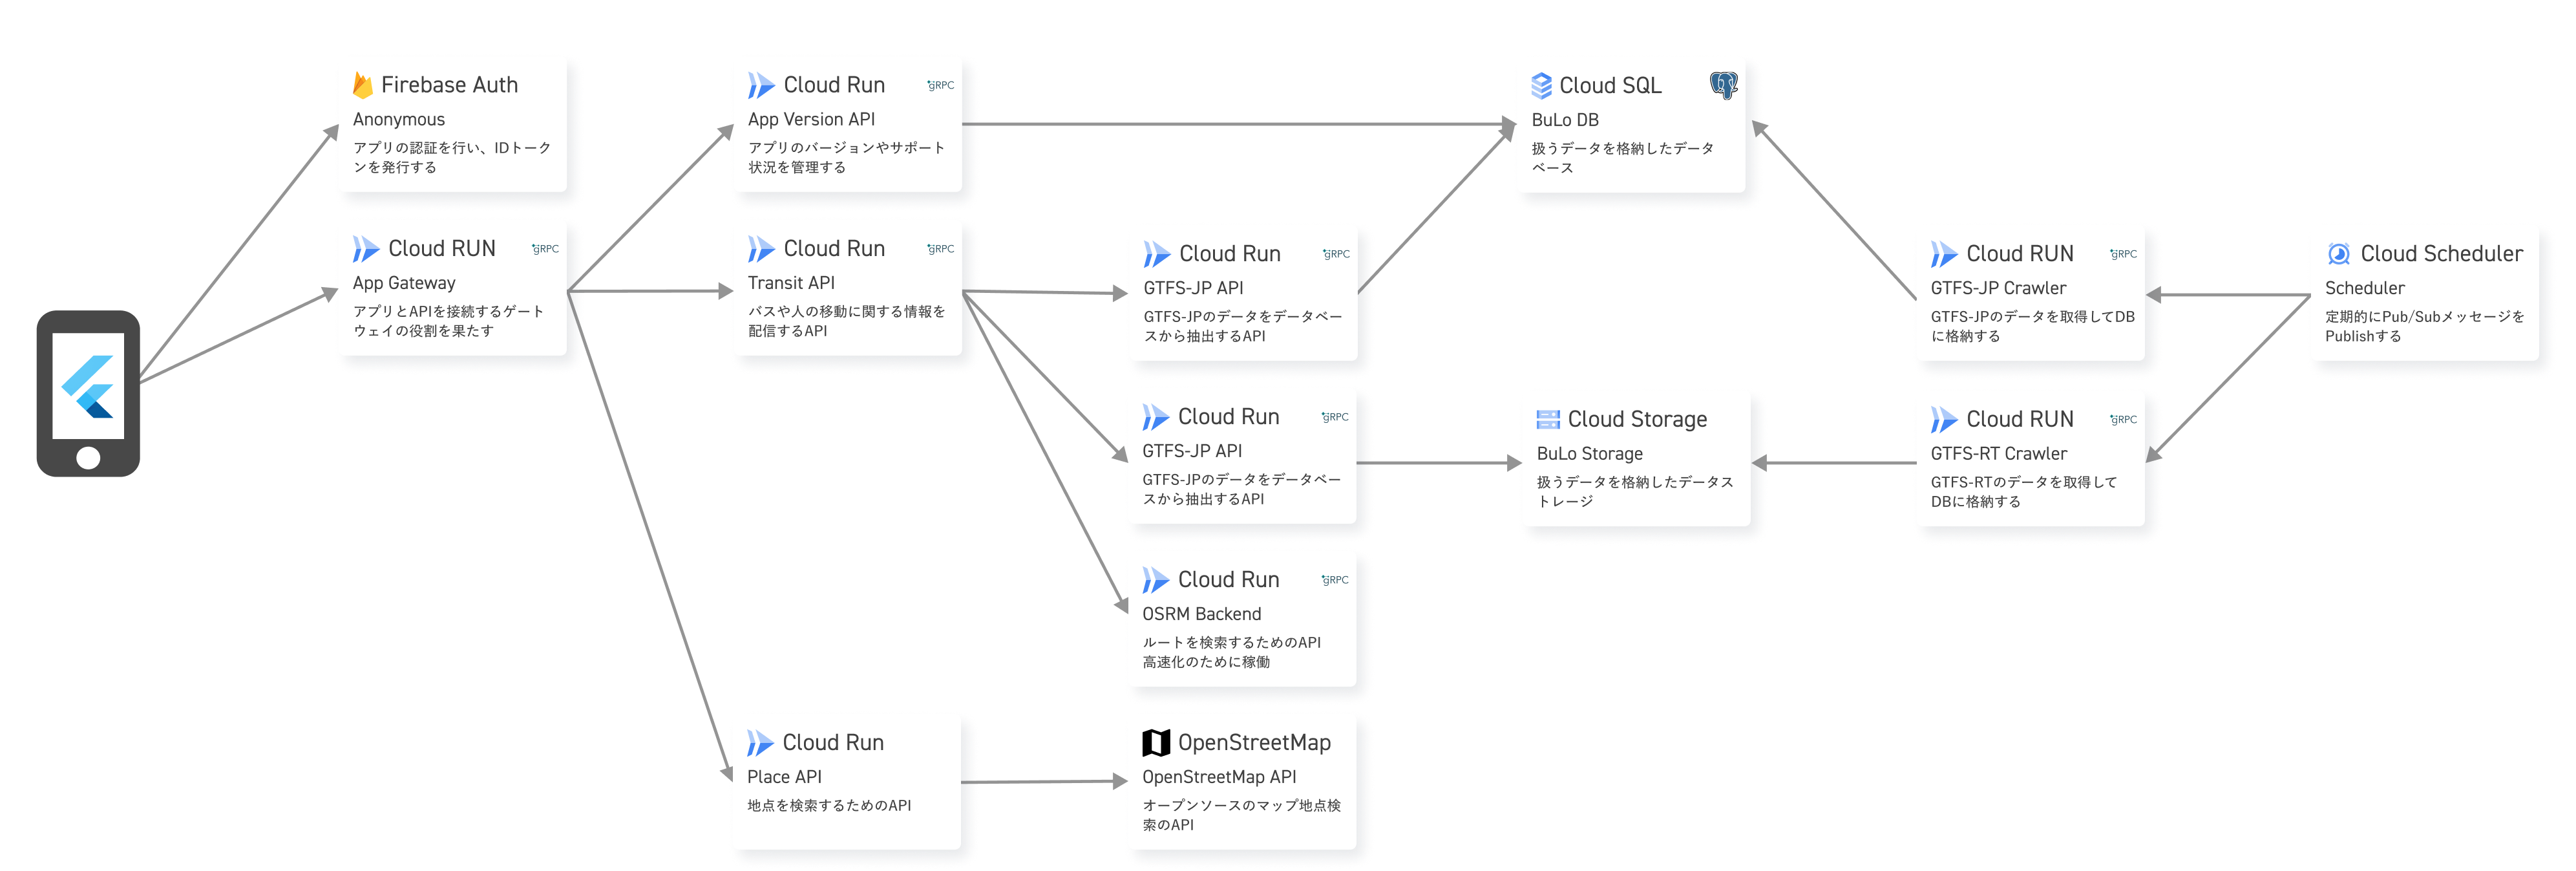
\includegraphics[width=14cm]{images/architecture_diagram.png}
    \caption{アーキテクチャ図}
    \label{fig:architecture}
\end{figure}
以下に,いくつかのマイクロサービスを抜粋して説明する.

\subsection{クライアントアプリケーション}
クライアントアプリケーションは,Flutter\footnote{https://flutter.dev/}を用いて開発した.Firebase Authentication\footnote{https://firebase.google.com/products/auth}を用いて,ユーザの匿名認証を行う.生成されたIDトークンを用いて,App Gatewayと通信をする.App Gatewayは,バックエンドのマイクロサービスと通信をして,クライアントが扱いやすい形で,データを返却する.高度なビジネスロジックをフロントエンド側で持たず,できる限りバックエンド側に切り出すようにした.

\subsection{Transit API}
本サービスで最も重要なマイクロサービスの1つである.クライアントアプリケーション内のTime-Distance ViewやRoute Viewを提供するために必要な情報を,GTFS-JP\footnote{https://www.gtfs.jp/}およびGTFS-RT\footnote{https://developers.google.com/transit/gtfs-realtime?hl=ja}のデータから計算する.

\subsection{Place API}
地点を検索する際に,入力されたキーワードから,マッチする地点を検索するマイクロサービスである.検索には,OpenStreetMap\footnote{https://www.openstreetmap.org/}のデータからジオコーディングを行う,Nominatim\footnote{https://nominatim.org/}というオープンソースのジオコーディングツールを使用した.
\bunseki{及川寛太}
